\section{Kompleksyfikacja} 
Ogólna idea: \\[0.25cm]
$\RR^n \to \CC^n$ \\ 
$M_{n \times n}(\RR) \to M_{n \times n}(\CC)$\\ 
$\RR \to \CC$ \\[0.5cm] 
Co dokładnie byśmy chcieli:\\[0.25cm]
$V - $ przestrzeń liniowa nad $\RR \to V_\CC - $ przestrzeń liniowa nad $\CC$ \\ 
$F: V \to V $ przekształcenie liniowe $\to F_\CC : V_\CC \to V_\CC$ \\ 
$V \subset V_\CC$ \\ 
jeśli $v,w \in V$, to $v +_\CC w = v + w$\\ 
jeśli $v \in V, \lambda \in \RR$, to $\lambda \cdot_\CC v = \lambda \cdot v$ \\ 
$F_\CC |_V = F$
\begin{df} 
    Kompleksyfikacją przestrzeni liniowej $V$ nad $\RR$ nazywamy przestrzeń liniową nad 
    $\CC$ zdefiniową następująco: 
    \begin{gather*} 
        V_\CC = \{ u + iv : u, v \in V \} \\ 
        (u + iv) + (u' + iv') = (u+u') + i(v +v') \\ 
        (a + ib) \cdot (u + iv) = (au - bv) + i(bu + av) \\ 
        a,b \in \RR,\ u,v \in V
    \end{gather*} 
\end{df} 
\begin{przy} ~\\
    Jeśli $V = \RR^n$, to $V_\CC = \CC^n$ \\ 
    Jeśli $V = \RR[x]$, to $V_\CC = \CC[x]$ \\ 
    Jesli $V = F(X,\RR)$, to $V_\CC = F(X,\CC)$
\end{przy} 
\begin{df} 
    Kompleksyfikacją przekształcenia liniowego $F: V \to V$ ($V - $ przestrzeń liniowa nad 
    $\RR$) nazywamy $F_\CC: V_\CC \to V_\CC$
    \[ F_\CC (u+iv) = F(u) + iF(v) \]
\end{df} 
\begin{ft} 
    $F_\CC$ jest $\CC - $ liniowe. 
\end{ft} 
\begin{dd} ~\\ 
    Należy sprawdzić addytywność: \\
    $F_\CC ((u+iv) + (u'+iv')) = F_\CC((u+u')+i(v+v')) = F(u+u') + iF(v+v') = 
    F(u) + F(u') + iF(v) + iF(v') = F_\CC (u+iv) + F_\CC(u' + iv')$ \\ 
    oraz jednorodność:  \\
    $F_\CC ((a+ib)(u+iv)) = F_\CC ((au-bv)+i(bu+av)) = F(au-bv)+iF(bu+av) = aF(u) - bF(v) 
    + ibF(u) + iaF(v) = a(F(u)+iF(v)) + ib(F(u)+iF(v)) = (a+ib) F_\CC (u+iv)$
\end{dd} 
\begin{ft} 
    Jeśli $b_1,\ldots,b_n \in V$ jest bazą $V$, to jest też bazą $V_\CC$
\end{ft} 
\begin{dd} ~\\ 
    generowanie: \\ 
    $V_\CC \ni u + iv = \sum \alpha_k + b_k + i\sum \beta_k + b_k = \sum (\alpha_k + 
    i \beta_k ) b_k$ \\ 
    lnz: $\sum (\alpha_k + i \beta_k) b_k = 0$ \\ 
    $ (\sum \alpha_k b_k) + i(\sum \beta_k b_k) = 0 \Rightarrow 
    \sum\alpha_k b_k = 0,\ \sum\beta_k b_k =0 \leftarrow$ a to już jest w $V$, czyli jedyna
    zerowa kombinacja liniowa jest $\forall k \ \alpha_k = \beta_k = 0 $
\end{dd} 
\begin{wn} $\dim_\CC (V_\CC) = dim_\RR (V)$ \end{wn} 
\begin{uw} $\dim_\CC (\CC^n) = n$, ale $\dim_\RR (\CC^n) = 2n$ \end{uw} 
\begin{wn} $V - $ rzecywista przestrzeń liniowa, $F: V \to V$ przekształcenie liniowe, to 
    $m_B^B (F) = m_B^B (F_\CC)$ \end{wn}
    \begin{df}[Fakt]
    Jeśli $(V,\scp \cdot \cdot) - $ przestrzeń euklidesowa (rzeczywista), to 
    $(V_\CC, \scp \cdot \cdot _\CC)$ jest przestrzenią euklidesową (zespoloną), gdzie:
    \[ \scp{u+iv}{u'+iv'}_\CC = \scp{u}{u'} + i\scp{v}{u'} - i\scp{u}{v'} + \scp{v}{v'}\]
\end{df} 
\begin{tw}[o postaci przekształcenia unitranego] ~\\
    Jeśli $U \in M_{n \times n} (\CC)$ jest unitarna, to $U = PDP^-1$, gdzie 
    $D - $ diagonalna, $P - $ unitarna. Wartości własne, co do modułu, sa równe $1$.
\end{tw} 
\begin{dd} był na ćwiczeniach \end{dd} 
\begin{tw}[o postaci przekształcenia ortogonalnego] ~\\ 
    Jeśli $A \in M_{n \times n}(\RR)$ jest ortogonalna, to 
    $A = P \begin{pmatrix} O_1 & & \\ & \ddots & \\ & & O_k \end{pmatrix} P^{-1}$, gdzie 
    $P$ - ortogonalna, a $O_i = \begin{pmatrix} \cos \theta_i & -\sin\theta_i
    \\ \sin \theta_i & \cos \theta_i \end{pmatrix}$ lub $O_i = (\pm 1)$
\end{tw} 
\begin{dd} ~\\ 
    $A \in M_{n \times n} (\RR)$ \\
    traktując $A$ jako macierz zespoloną dostajemy rozkład: 
    $A = P \begin{pmatrix} \lambda_1 & & \\ &\ddots& \\ & & \lambda_n \end{pmatrix}P^{-1}$
    \\$A = P \begin{pmatrix} 1 & & & & & & & & \\ 
                           & \ddots & & & & & & & \\ 
                           & & 1 & & & & & & \\ 
                           & & & -1 & & & & & \\ 
                           & & & & \ddots & & & &  \\ 
                           & & & & & -1 & & & \\ 
                           & & & & & & a_1 + ib_1 & & \\ 
                           & & & & & & & a_1 - ib_1 &  \\
                           & & & & & & & & \ddots 
           \end{pmatrix} P^{-1}$ \\ 
           $P=(\underbrace{b_1,\ldots,b_p}_{\text{dla} \pm 1},b_{p+1},\overline{b_p{+1}},\ldots)$ \\ 
        $\begin{pmatrix} & \\ u+iv & u - iv \\ & \end{pmatrix} 
        \begin{pmatrix} a + ib & \\ & a - ib \end{pmatrix} \begin{pmatrix} & \\ & 
    \end{pmatrix}^{-1}$ 
    $ \operatorname{Lin} \{u,v\} = \operatorname{Lin} \{b_{p+1}, \overline{b_{p+1}}\}$ \\ 
    $A (u+iv) = (a+ib)(u+iv)$ \\ 
    $A (u-iv) = (a-ib)(u-iv)$ \\ 
    $Au \pm Av = (au - bv) \pm i(bu+av)$ \\ 
    $Au = au - bv $ \\ 
    $Av = bu + av $ \\ 
    $\begin{pmatrix} a + ib & \\ & a - ib \end{pmatrix} 
    \to \begin{pmatrix} a & b \\ -b & a \end{pmatrix}$ \\ 
    $a^2 + b^2 = 1$, czyli $a = \cos \theta,\ b = -\sin\theta$
\end{dd} 
\begin{tw}[Jordana (wersja rzeczywista)] 
$A \in M_{n \times n}(\RR)$ \\ 
Wówczas $A = PJP^{-1}$, gdzie $J = \begin{pmatrix} J_1 & & \\ & \ddots & \\ & & J_n 
    \end{pmatrix}$, gdzie \\
    $J_i = \begin{pmatrix} \lambda_i \end{pmatrix},\ \lambda_i \in \RR$ \\ 
    lub \\ 
    $J_i = \begin{pmatrix} \lambda_i & 1 & & & \\ 
                           & \ddots & \ddots & & \\ 
                           & & \ddots & 1 &  \\
                           & & & \lambda_i 
    \end{pmatrix},\ \lambda_i \in \RR$ \\ 
    lub \\ 
    $J_i = 
    \begin{pmatrix} a_i & -b_i \\ b_i & a_i \end{pmatrix} a_i, b_i \in \RR$ \\ 
    lub \\
    $J_i = 
    \begin{pmatrix} 
        a_i & -b_i& 1      & 0      & &  \\ 
        b_i & a_i & 0      & 1      & &  \\ 
            & \ddots    &  & \ddots & &  \\ 
            &     &  \ddots  &  & 1 & 0 \\
            &     &        & \ddots& 0 & 1 \\ 
            &     &        & & a_i &  -b_i \\ 
            &     &        & & b_i & a_i
    \end{pmatrix}$ 
\end{tw} 
\begin{dd} 
    $A = PJP^{-1}$ - rozkład zespolony (dbając o to, by wektory bazowe dla rzeczywistych
    wartości własnych były rzeczywiste) \\ 
    $ \lambda \notin \RR$ \\ 
    $ \lambda, \overline \lambda$ \\ 
    $\overline {V_\lambda} = V_{\overline\lambda}$ \\ 
    $\overline{\ker (A-\lambda I)^n} = \ker (A - \overline\lambda I) \to $ klatka dla 
    $\lambda$ są takie same co dla $\overline \lambda$ \\ 
    Jeśli skonstruujemy kawałek bazy jordanowskiej $b_1,\ldots,b_n$ dla $\lambda$, to 
    $\overline b_1,\ldots,\overline b_n$ będą odpowiednio kawałekiem bazy jordanowskiej dla
    $\overline \lambda$. \\ 
    Następnie powtarzamy procedurę z poprzedniego twierdzenia. \\ 
    $b_1,\ldots,b_n,\overline b_1,\ldots,\overline b_n \to 
    \operatorname{Re} b_1, \operatorname{Im} b_1,\ldots,\operatorname{Re}b_n,
    \operatorname{Im} b_n$ 
\end{dd} 
\section{Objętość n-wymiarowa}
Znakowana objętosć $n-$wymiarowego równoległościanu rozpiętego przez wektory 
$v_1,\ldots,v_n \in \RR^n$
\begin{df}[tw] 
    Objętością $n-$ wymiarowego rownoległościanu rozpiętego przez $v_1,\ldots,v_n \in \RR^n$ 
    nazywamy każdą z poniżej podanych (równych) liczb. 
    \begin{enumerate}[(1)] 
        \item $|\det(v_1,\ldots,v_n)|$
        \item $V_n$, gdzie $\begin{cases} V_1 = |v_1| \\ 
                V_{k+1} = V_k * \operatorname{dist}
            (v_{k+1},\operatorname{Lin} \{v_1,\ldots,v_n \}) \end{cases}$
        \item $\sqrt{\det\begin{pmatrix} \scp{v_1}{v_1}&\ldots&\scp{v_1}{v_n} \\ 
                    & \vdots & \\ 
            \scp{v_n}{v_1} & \ldots & \scp{v_n}{v_n} \end{pmatrix}}$ macierz Grama
    \end{enumerate} 
\end{df} 
\begin{dd} ~
    \begin{itemize} 
    \item[$(1) \Leftrightarrow (3)$] 
        $\begin{pmatrix} \scp{v_1}{v_1} & \ldots & \scp{v_1}{v_n} \\ 
            & \vdots & \\ 
        \scp{v_n}{v_1} & \ldots & \scp{v_n}{v_n} \end{pmatrix} = 
        \begin{pmatrix} v_1^\top \\ \vdots \\ v_n^\top \end{pmatrix} 
        \begin{pmatrix} v_1 & \ldots & v_n \end{pmatrix} $ \\ 
        $G = A^\top A$ \\ 
        $\det G = \det A^\top \det A = (\det A)^2$
    \item[$(2) \Leftrightarrow (1)$] Zastosowanie ortogonalizacji Grama-Schmidta do $v_1,
        \ldots,v_n$ nie wpływa na wartość $V_n$.  \\ 
    Nie wpływa również na $\det(v_1,\ldots,v_n)$  \\ 
    Zatem wystarczy sprawdzić dla układu ortogonalnego. Wtedy: 
    $\det(v_1,\ldots,v_n) = (det(\scp{v_i}{v_j}))^{\frac{1}{2}} = \\ 
    \sqrt{|v_1|^2\ldots|v_n|^2} = |v_1|\ldots|v_n| = V_n$
    \end{itemize} 
\end{dd} 
\begin{wn} Objętość nie zależy od kolejności wektorów \end{wn} 
\begin{dd} Zamiana kolumn w macierzy $(v_1,\ldots,v_n)$ zmienia jedynie znak wyznacznika. 
\end{dd} 
\begin{wn} Objętość wynosi $|\det([v_1]_B,\ldots,[v_n]_B)|$, gdzie $B$ jest dowolną bazą 
ortonormalną \end{wn} 
\begin{dd} taki sam \end{dd} 
\begin{wn} $v_1,\ldots,v_n \in \RR^n$ lnz $\Leftrightarrow \det(\scp{v_i}{v_j}) \neq 0$
\end{wn} 
\section{Przestrzeń dualna} 
\begin{df} 
    $V - $ przestrzeń liniowa nad $K$ \\ 
    Przestrzenią dualną do $V$ nazywamy $V^* = \operatorname{Hom} (V,K)$ (elementy 
    $V^*$ nazywamy czasami funkcjonałami (liniowymi))
\end{df} 
\begin{ft} 
    Jesli $\dim V < \infty$, to $V^* \simeq V$
\end{ft} 
\begin{dd} 
    $b_1,\ldots,b_n - $ baza $V$ \\ 
    $b_1^*,\ldots,b_n^* \in V^*$ (baza dualna), $ b_i^* (b_j) = 
    \begin{cases} 1, & i = j \\ 0, & i \neq j \end{cases}$ \\
    Dalej rozszerzamy do liniowego $b_i^* V \to K$ \\ 
    (inaczej $b_i^* (\alpha_1 b_1 + \ldots + \alpha_n b_n) = \alpha_i$) \\ 
    generowanie: \\ 
    $v^* \in V^* \quad (v^* : V \to K)$ \\ 
    $ v^* \overset{?}{=} v^*(b_1) b^*_1 + \ldots v^*(b_n) b^*_n$ \\ 
    sprawdzimy, czy oba odwzorowania są zgodne na bazie $b_1,\ldots,b_n$  \\ 
    $v^* (b_j) = v^*(b_1) \underbracket{b_1^*(b_j)}_{0} + \ldots + 
    v^*(b_n) \underbracket{b_n^* (bj)}_{0}$ \\ 
    lnz: \\ 
    $\alpha_1 b-1 ^* + \ldots + \alpha_n b_n^* = 0$ \\ 
    $\alpha_1 b_1 ^* (b_j) + \ldots + \alpha_n b_n^*(b_j) = 0$ \\ 
    $\alpha_j = 0$ dla $j = 1,\ldots,n$ \\ 
    zatem $dim V^* = \dim V < \infty$, czyli $V^* \simeq V$ 
\end{dd} 
\begin{uw} ~\\  
    $V = \RR^\infty = 
     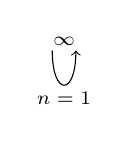
\begin{tikzpicture}[scale = 0.3,baseline]
        \node at (0.5,1.4) {\scriptsize$\infty$};
        \node at (0.5,-1) {\scriptsize$n=1$};
        \path[->] (0,1) edge [bend right = 90,looseness=5] (1,1);
    \end{tikzpicture} \  
    \RR^n$ \\ 
    $V^* \simeq V$ 
\end{uw} 
\begin{df} 
    $F: V \to W$ przekształcenie liniowe, to przekształcenie dualne do $F$, 
    to $F^*: W^* \to V^*$, takie, że $F^*(w^*) = w^* \circ F$
\end{df} 
\begin{ft} 
    Odwozorowanie $\varphi: V \to V^{**}$ zdefiniowane $\varphi(v)(f) = f(v)$ jest 
    monomorfizmem. W przypadku $\dim V < \infty $ jest to izomorfizm. 
\end{ft} 
\footnotetext{monomorfizm - różnowartościowe \\ epimorfizm - na \\ 
endomorifzm $V \to V$ \\ automirfozim = endo + izo}
$V^{**} = (V^*)^*$ 
$\varphi (v) \in (V^*)^*$ \\ 
$\varphi (v): V^* \to K$ \\ 
$\varphi (v) (f) = f(v)$ \\ 
$f: V \to K$
